\documentclass{article}\usepackage[]{graphicx}\usepackage[]{color}
%% maxwidth is the original width if it is less than linewidth
%% otherwise use linewidth (to make sure the graphics do not exceed the margin)
\makeatletter
\def\maxwidth{ %
  \ifdim\Gin@nat@width>\linewidth
    \linewidth
  \else
    \Gin@nat@width
  \fi
}
\makeatother

\definecolor{fgcolor}{rgb}{0.345, 0.345, 0.345}
\newcommand{\hlnum}[1]{\textcolor[rgb]{0.686,0.059,0.569}{#1}}%
\newcommand{\hlstr}[1]{\textcolor[rgb]{0.192,0.494,0.8}{#1}}%
\newcommand{\hlcom}[1]{\textcolor[rgb]{0.678,0.584,0.686}{\textit{#1}}}%
\newcommand{\hlopt}[1]{\textcolor[rgb]{0,0,0}{#1}}%
\newcommand{\hlstd}[1]{\textcolor[rgb]{0.345,0.345,0.345}{#1}}%
\newcommand{\hlkwa}[1]{\textcolor[rgb]{0.161,0.373,0.58}{\textbf{#1}}}%
\newcommand{\hlkwb}[1]{\textcolor[rgb]{0.69,0.353,0.396}{#1}}%
\newcommand{\hlkwc}[1]{\textcolor[rgb]{0.333,0.667,0.333}{#1}}%
\newcommand{\hlkwd}[1]{\textcolor[rgb]{0.737,0.353,0.396}{\textbf{#1}}}%
\let\hlipl\hlkwb

\usepackage{framed}
\makeatletter
\newenvironment{kframe}{%
 \def\at@end@of@kframe{}%
 \ifinner\ifhmode%
  \def\at@end@of@kframe{\end{minipage}}%
  \begin{minipage}{\columnwidth}%
 \fi\fi%
 \def\FrameCommand##1{\hskip\@totalleftmargin \hskip-\fboxsep
 \colorbox{shadecolor}{##1}\hskip-\fboxsep
     % There is no \\@totalrightmargin, so:
     \hskip-\linewidth \hskip-\@totalleftmargin \hskip\columnwidth}%
 \MakeFramed {\advance\hsize-\width
   \@totalleftmargin\z@ \linewidth\hsize
   \@setminipage}}%
 {\par\unskip\endMakeFramed%
 \at@end@of@kframe}
\makeatother

\definecolor{shadecolor}{rgb}{.97, .97, .97}
\definecolor{messagecolor}{rgb}{0, 0, 0}
\definecolor{warningcolor}{rgb}{1, 0, 1}
\definecolor{errorcolor}{rgb}{1, 0, 0}
\newenvironment{knitrout}{}{} % an empty environment to be redefined in TeX

\usepackage{alltt}
\usepackage[top=1.00in, bottom=1.0in, left=1.1in, right=1.1in]{geometry}
\renewcommand{\baselinestretch}{1.1}
\usepackage{graphicx}
\usepackage{natbib}
\usepackage{amsmath}
\bibliographystyle{..//refs/styles/besjournals.bst}
\renewcommand{\thetable}{S\arabic{table}}
\renewcommand{\thefigure}{S\arabic{figure}}
\usepackage{xr-hyper}
\externaldocument{shortest_reconciling}

\def\labelitemi{--}
\parindent=24pt
\title{Supplement: Reconciling competing hypotheses regarding flower-leaf sequences in temperate forests for fundamental and global change biology}
\IfFileExists{upquote.sty}{\usepackage{upquote}}{}
\begin{document}
\maketitle

\subsection*{Methods}
\subsubsection*{Climate Change and FLS:}
To evaluate how FLS patterns have changed over time in association with climate change we obtained phenological data for four European woody plant species with long term phenology records of both flower (BBCH 60) and leafout phenology (BBCH 11) from the Pan European Phenological Database \citep{PEP725}. We restricted the data set to include only stations with more than 50 years worth of data. Following conventions for modeling effects of climate change, we modeled the number of days between flowering and leafing as a function of time for each species, using a hinge model with 1980 as a break point \citep{IPCC2013,Kharouba2018}. For each species, we display the pre-1980 mean and 95\% credible intervals of the time between flowering and leafing and the post-1980 change in mean time between phenophases that can be driven by climate change.

\subsubsection*{Defining FLS with MTSV and USFS data}
For these two, categorical, species level-case studies, we converted verbal descriptions of flower-leaf sequences into a binary response variable. For our more inclusive ``functional" definition of hysteranthy, which allows for some overlap between floral and vegetative phenophases, we included species entries with descriptions \textit{``flowers before the leaves"}, \textit{``flowers before or with leaves"} and \textit{``flowers with leaves"} as hysteranthous. Our more restrictive ``physiological" hysteranthy definition only included species described as \textit{``flowers before the leaves"} as hysteranthous.\\

\noindent For modeling trait associations with FLS, we chose three predictors to represent the three major FLS hypotheses; pollination syndrome, average flowering time and minimum precipitation levels across the species range. We obtained pollination syndrome and average flowering time information directly from the respective data sources and estimates of minimum precipitation across range from the USDA/NRCS Conservation Plants Characteristics database \citep{NRCS}. We coded pollination syndrome as biotic- or wind-pollinated, and assigned known ambophilous species in the genus \textit{Salix} as biotic-pollinated. We re-coded flowering time as the average of the range of months of flowering reported in each data source.\\

\noindent For these case studies, we modeled associations between hysteranthy and the trait predictors with logistical regressions in phylogenetic generalized linear modeling framework \citep{Ives2010} using the R package ``phylolm" \citep{Ho2014}. Our models incorporated a published angiosperm phylogenetic tree \citep{Zanne2013} pruned to match the species list for each case study. Species found in the trait data set but not in the original phylogenetic tree were added to the pruned tree at the generic root. In total 32 species were added to the generic roots for the MTSV data set and eight for the USFS data set. We visualize phylogenetic patterning of FLS across the tree of each case study (Fig. \ref{fig:phylogeny}).\\

\noindent We ran the models with 599 bootstrapped re-sampling iterations for each data set \citep{Wilcox2010}. We standardized all predictors by subtracting the mean and dividing by two standard deviations to allow for a reasonable comparison of effect sizes between the binary and continuous predictors in this model \citep{Gelman2007}. 



\subsubsection*{Harvard Forest models}
For each individual tree per year in the data, we calculated the time between flowers opening and leaves reaching 75\% of their final size. Positive FLS values indicate flowering-first and negative values leafing-first. To compare the inference between categorical and continuous measure of FLS, we re-coded the continuous FLS measures as binary responses with positive values coded as hysteranthous and negative values as seranthous. These models used the same predictors as the MTSV and USFS datasets, except that we estimated flowering time directly from the HF data. All models the R package ``brms" \citep{Burkner2018} to estimate the relationship between FLS and the predictors with a phylogenetic mixed model in a Bayesian framework \citep{Garamszegi2014}. We ran 4 chains with 4000 iterations and a
warm-up of 3000 iterations each, resulting in 4000 total sampling iteration. All models used weakly informative priors. As our primary goal was to directly compare the effects each predictor, we standardized these variables to allow for a reasonable comparison between them {\citep{Gelman2007}. \\

\noindent To examine the relationship between inter-annual variation in FLS and precipitation, we obtained precipitation records from the Shaler meteorological station at Harvard Forest \citep{Boose2004}. As above, these models run with weak priors, a warm up of 3000 iterations and 4000 sampling iterations.\\

\noindent The three Harvard Forest models are detailed below:\\
\begin{enumerate}
\item \underline{Categorical model}:\\
Pr(y_i &=1) &= logit^{-1} \alpha_{sp[i]} + \alpha_{phylo[i]} + \beta_{pollination syndrome}X_1_[_i_] + \beta_{flowering time}X_2_[_i_] + \beta_{min. precipitation}X_3_[_i_] +\beta_{pollination syndrome}:\beta_{flowering time}X_4_[_i_]+\beta_{pollination syndrome}:\beta_{min. precipitation}X_5_[_i_]+ \beta_{flowering time}:\beta_{min. precipitation}X_6_[_i_] + \epsilon_i\\

\epsilon_i & \sim N(0,\sigma^2_y) \\ 

\noindent The influence of the phylogeny $\alpha_phylo$ was modeled as follows:\\
\alpha_{sp} & \sim N(\mu_{\alpha}, COR[\sigma^2_{phylo}]) \\

\noindent THe $\alpha$ for species effects indendent of the phylogeny was modeled as follows:\\
\alpha_{sp} & \sim N(\mu_{\alpha}, \sigma^2_{species}) \\

\item \underline{Continuous model}: \\
y_i &= \alpha_{ind/sp[i]} +\alpha_{phylo[i]} + \beta_{pollination syndrome}X_1_[_i_] + \beta_{flowering time}X_2_[_i_] + \beta_{min. precipitation}X_3_[_i_] +\beta_{pollination syndrome}:\beta_{flowering time}X_4_[_i_]+\beta_{pollination syndrome}:\beta_{min. precipitation}X_5_[_i_]+ \beta_{flowering time}:\beta_{min. precipitation}X_6_[_i_] + \epsilon_i\\

\epsilon_i & \sim N(0,\sigma^2_y) \\ %I Think this is wrong and should reflect the phyogeny


\noindent The effect of the phylogeny was model as above and here, the individual effects within species were modeled:\\
\alpha_{ind/sp} & \sim N(\mu_{\alpha}, \sigma^2_{ind/sp}) \\

\item \underline{Inter-annual model}:\\
y_i &= \alpha_{i} + \beta_{annual precipitation}X_1[_i_] + \epsilon_i\\
\epsilon_i & \sim N(0,\sigma^2_y) \\

\end{enumerate}
\indent We calculated the marginal effects for the Harvard Forest continuous model using the R-package ``ggeffects" \citep{Ludecke2018}.\\

\noindent Though we make broad comparisons between the HF and MTSV/USFS case studies, differences in data structure between the datasets required us to use alternative modeling frameworks. The MTSV and USFS data provide one response variable for each species while the HF data contains intra-specific differences in FLS, providing several different response values per species. The current phylogenetic generalized linear model framework can only fit models with one response value per species, while the phylogenetic mixed model in brms over-fits models with this kind of data structure (Paul Burkner, personal communication) and performs better on multi-response per species datasets like HF. We ran both model types on each case study and while they do yield different absolute estimates, the patterns we found were consistent across each framework, and we report results from the most accurate model for each dataset.\\

\subsubsection*{Phylogenetic signals}
For all categorical specifications of FLS (MTSV, USFS and HF), we assessed the phylogenetic structure of hysteranthous flowering in all  with Fritz's D-statistic \citep{FRITZ2010} using the ``Caper" package \citep{Orme2013} in R. Fritz's D calculates the sum of changes in estimated node values of a binary trait along edges in a phylogeny and compares this observed value to both a model of Phylogenetic randomness and Brownian threshold model. The means of the two data simulations scale values of D to set points of 0 (as phylogenetically conserved) and 1 (random)  \citep{Orme2013}.\\

\noindent For the quantitative Harvard Forest model, we estimated the phylogenetic signal for FLS (lambda) based  covarience of residuals among species. Estimated phylogenetic signals from all case studies are reported below (Fig. \ref{fig:Dstat})  % I can probabalby elaborate on this. 

\section*{Supplemental Tables and Figures}

\begin{figure}[h!]
    \centering
 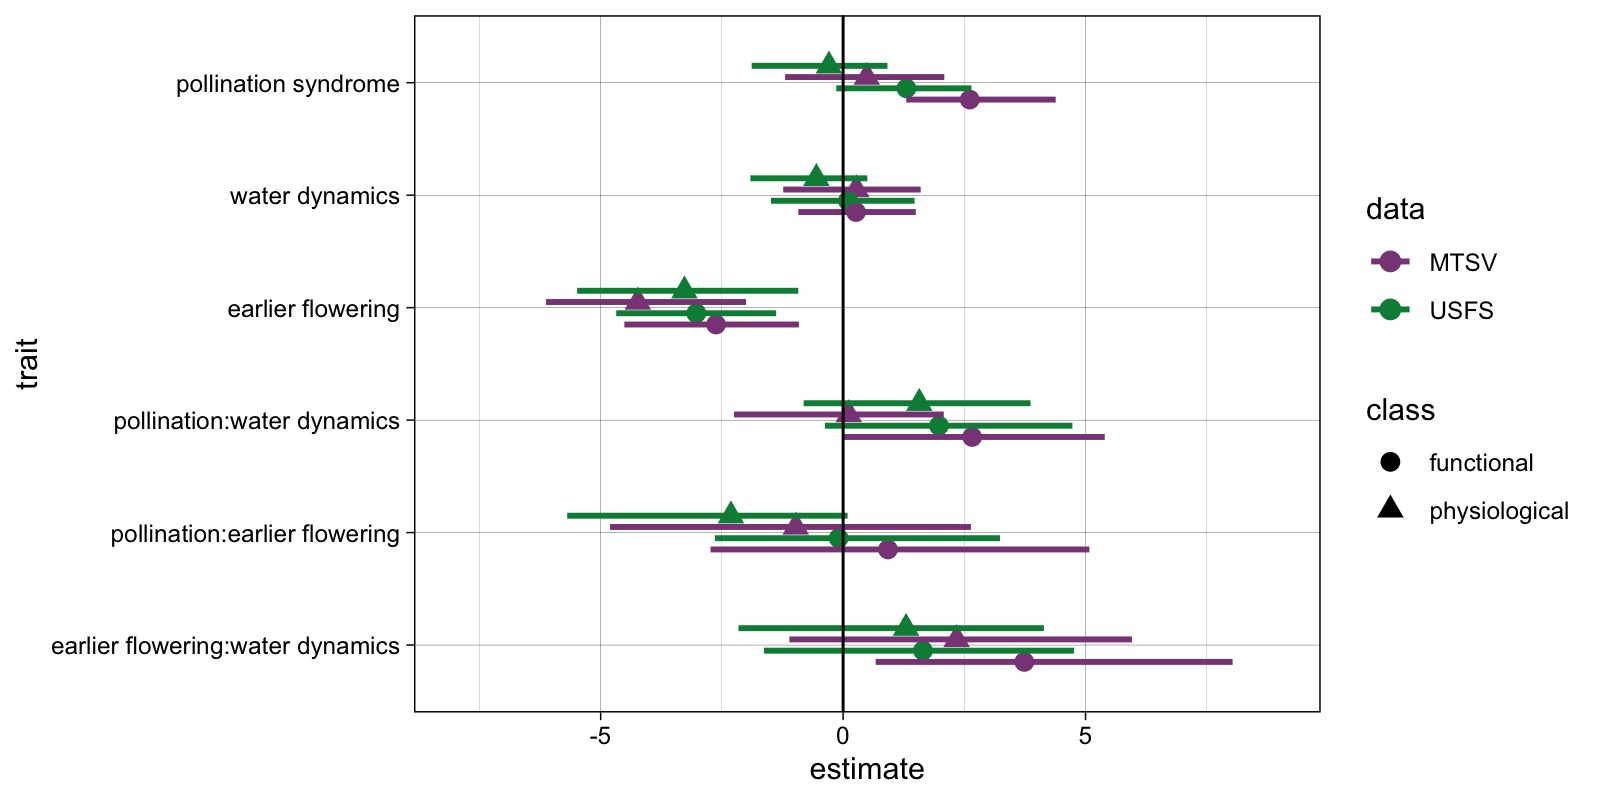
\includegraphics[width=\textwidth]{..//MTSV_USFS.jpeg} 
    \caption{\textbf{Mean estimates of the effects of FLS predictors on the likelihood a species is hysteranthous vary across datasets and definitions of FLS.}  We used phylogenetic adjustments and standardized units to make a basic comparison of two datasets and classes (physiological= no overlap between flowering and leafing, functional= moderate overlap) of FLS. While there is some agreement across models (strong effects of flowering time, no consistent effect interactions between predictors), the effect of other predictors (pollination syndrome, water dynamics) were highly sensitive to how data were defined, biasing any inference from models and compromising the ability to validate the existing FLS hypotheses. Lines represent 95\% bootstrap intervals.}
    \label{fig:muplots.USMT}
\end{figure}

\begin{figure}[h!]
    \centering
 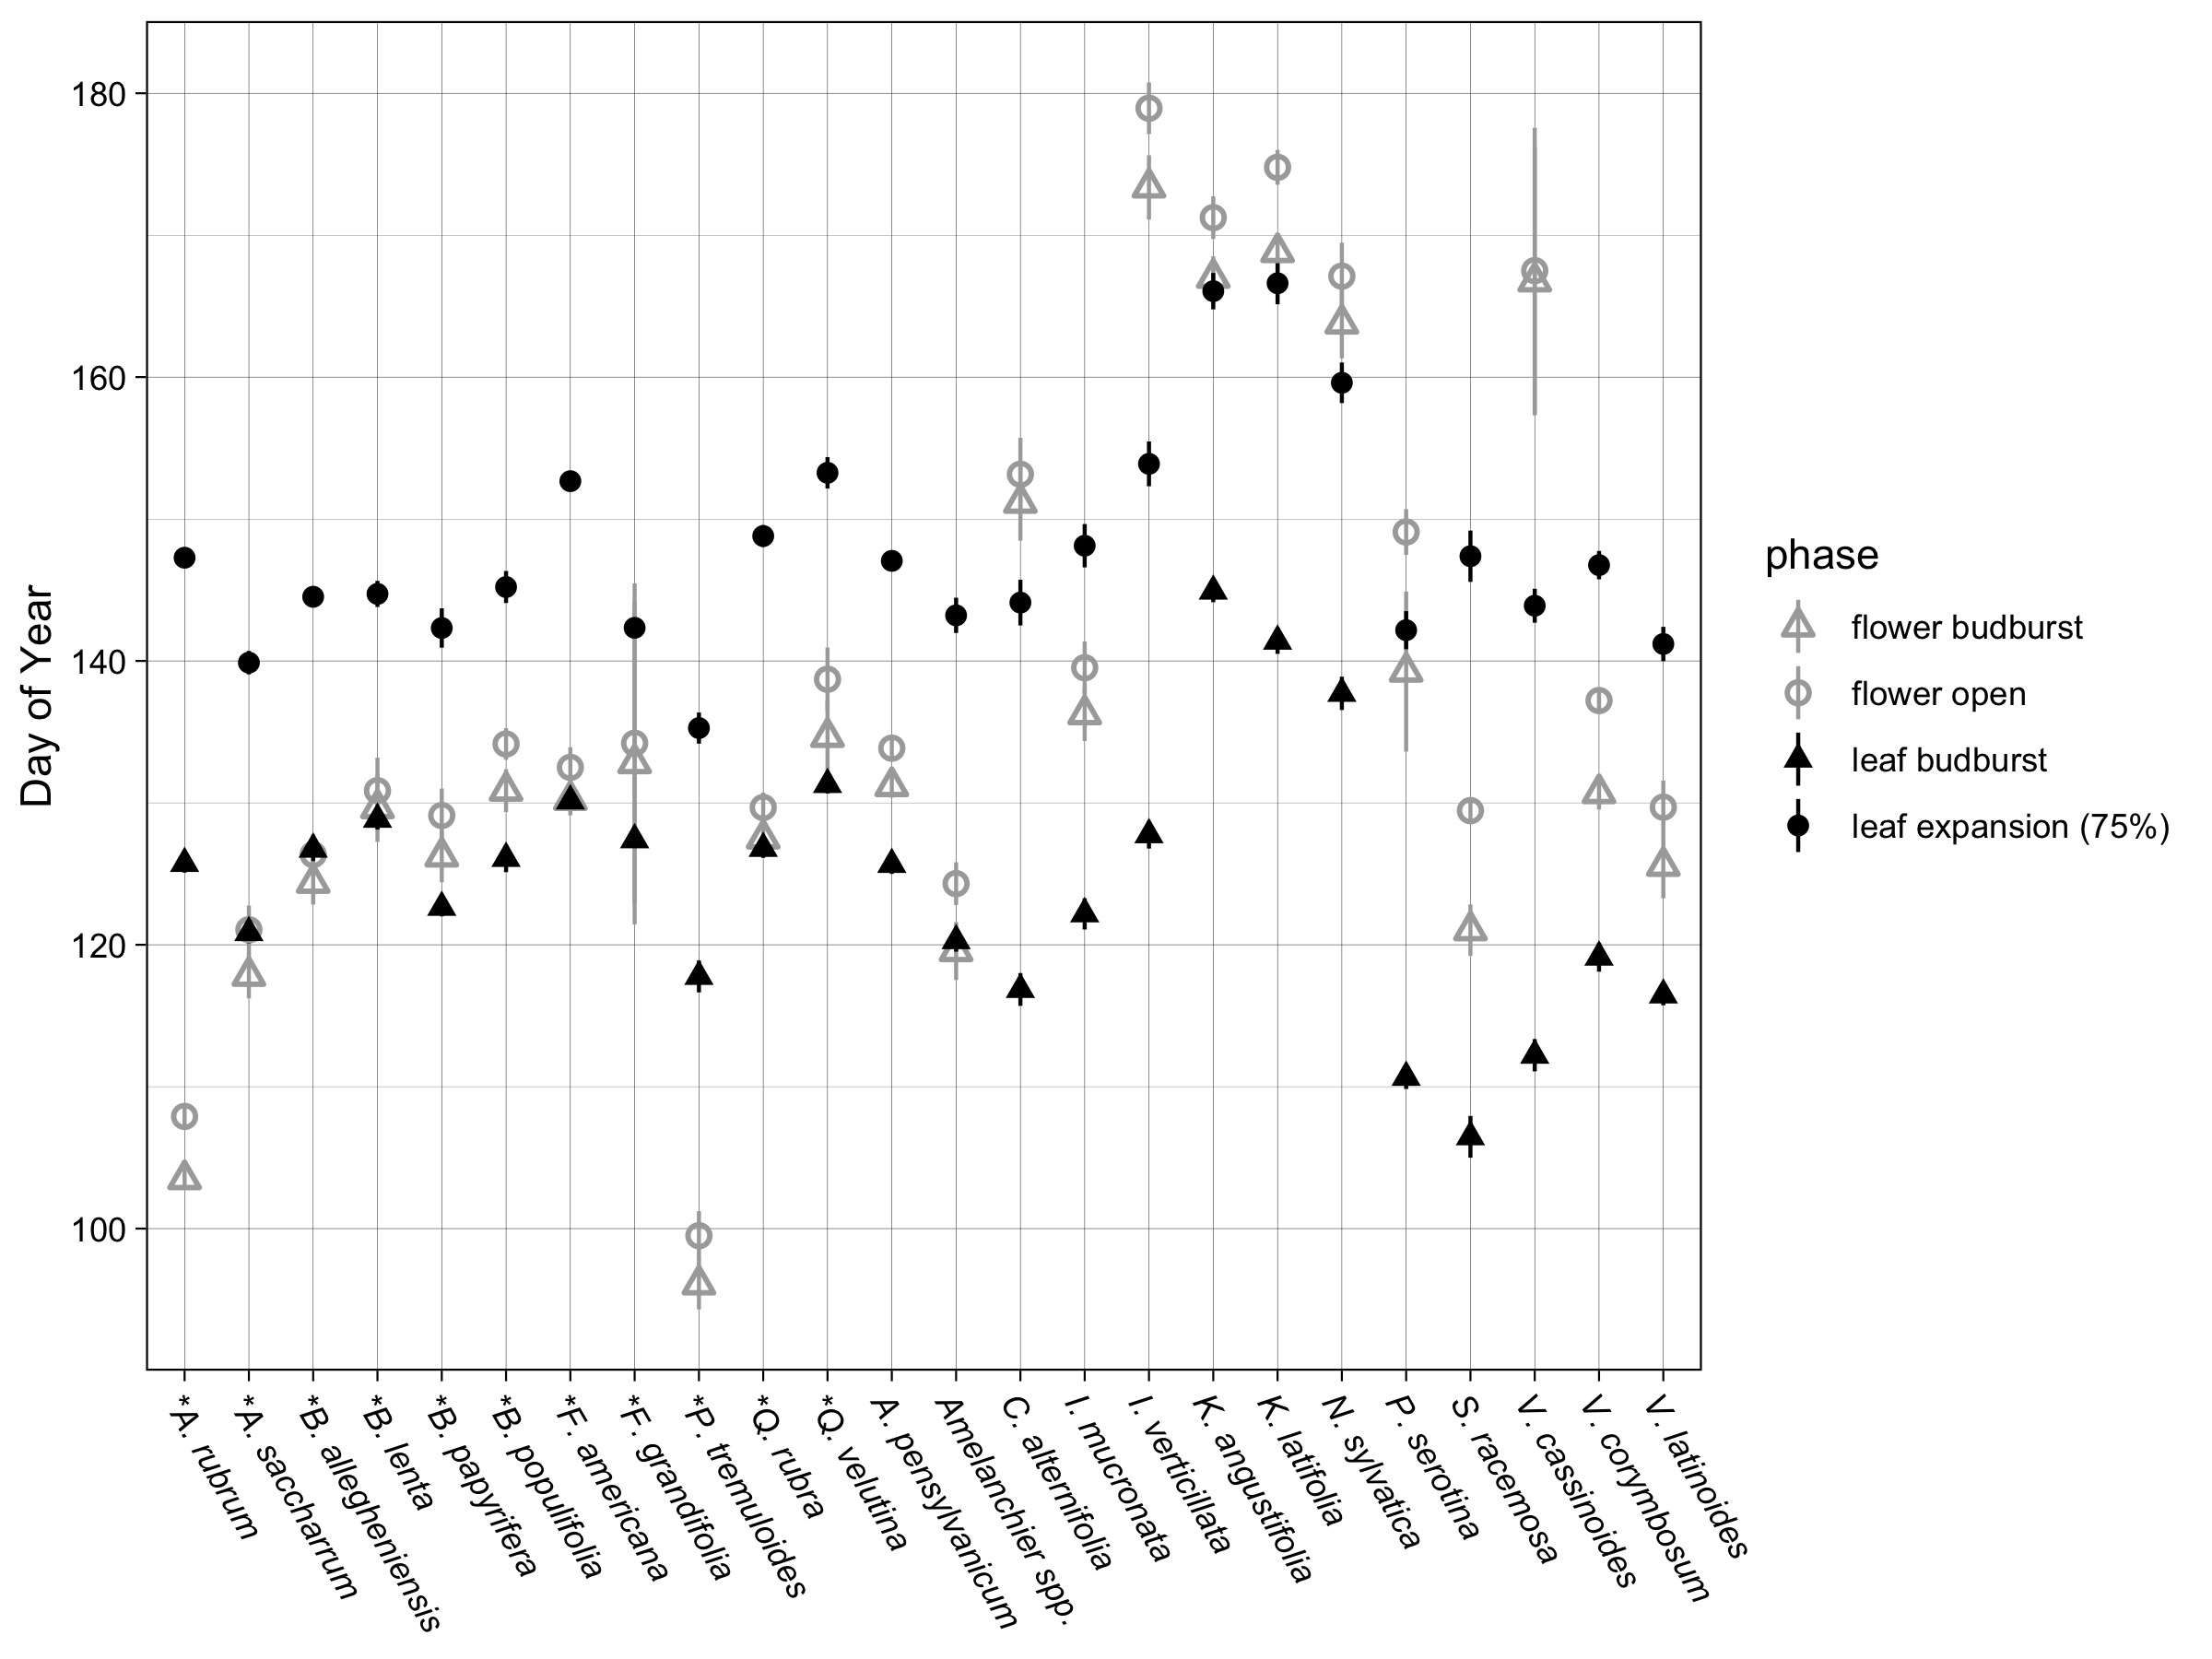
\includegraphics[width=\textwidth]{..//HarvardForest/HFmeans_expanded.jpeg} 
    \caption{\textbf{Quantitative FLS patterns for woody plants at Harvard Forest in Pertersham, MA.} Because phenological sequences consist of several sub-stages if is difficult to unambiguously categorize many species into the currently FLS categories. }
    \label{fig:HFmeans}
\end{figure}

\begin{figure}
 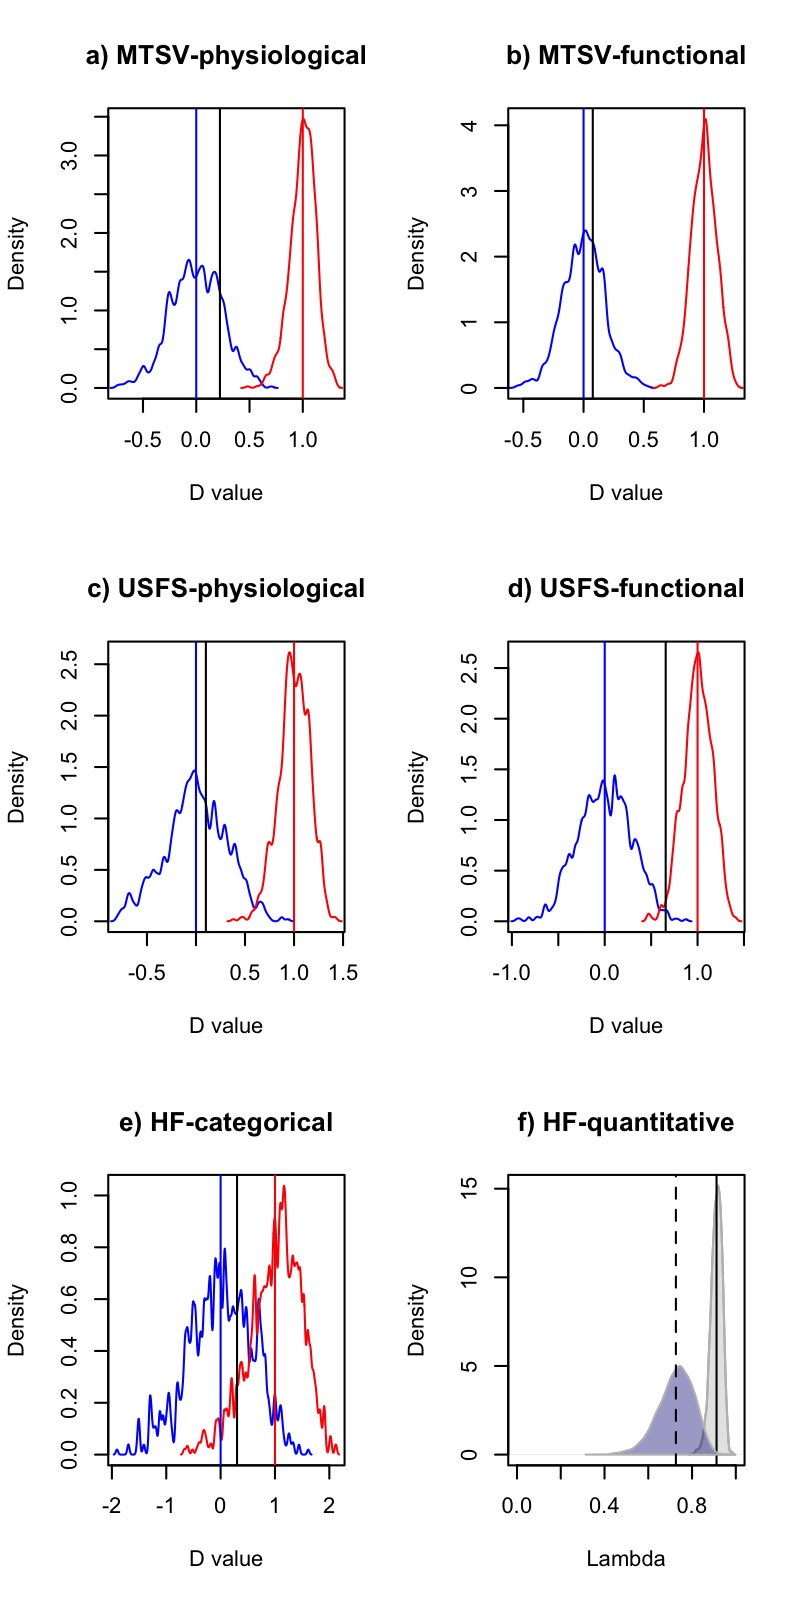
\includegraphics[height=0.9\textheight]{..//phylosig.jpeg} 
  \caption{\textbf{The phylogenetic signal for FLS varies between datasets, and is sensitive to how FLS patterns are categorized.} In a)-e),the black vertical line show the the Fritz's D statistic for binary classifications of FLS estimated from the data, with blue and red lines representing expected D values based on simulations under Brownian threshold model and random model respectively. Panel f) shows the the estimated $\lambda$ values of FLS from the the continuous modeling framework. Higher values indicate stronger phylogenetic structure.}
    \label{fig:Dstat}
    \end{figure}

\begin{figure}[H]

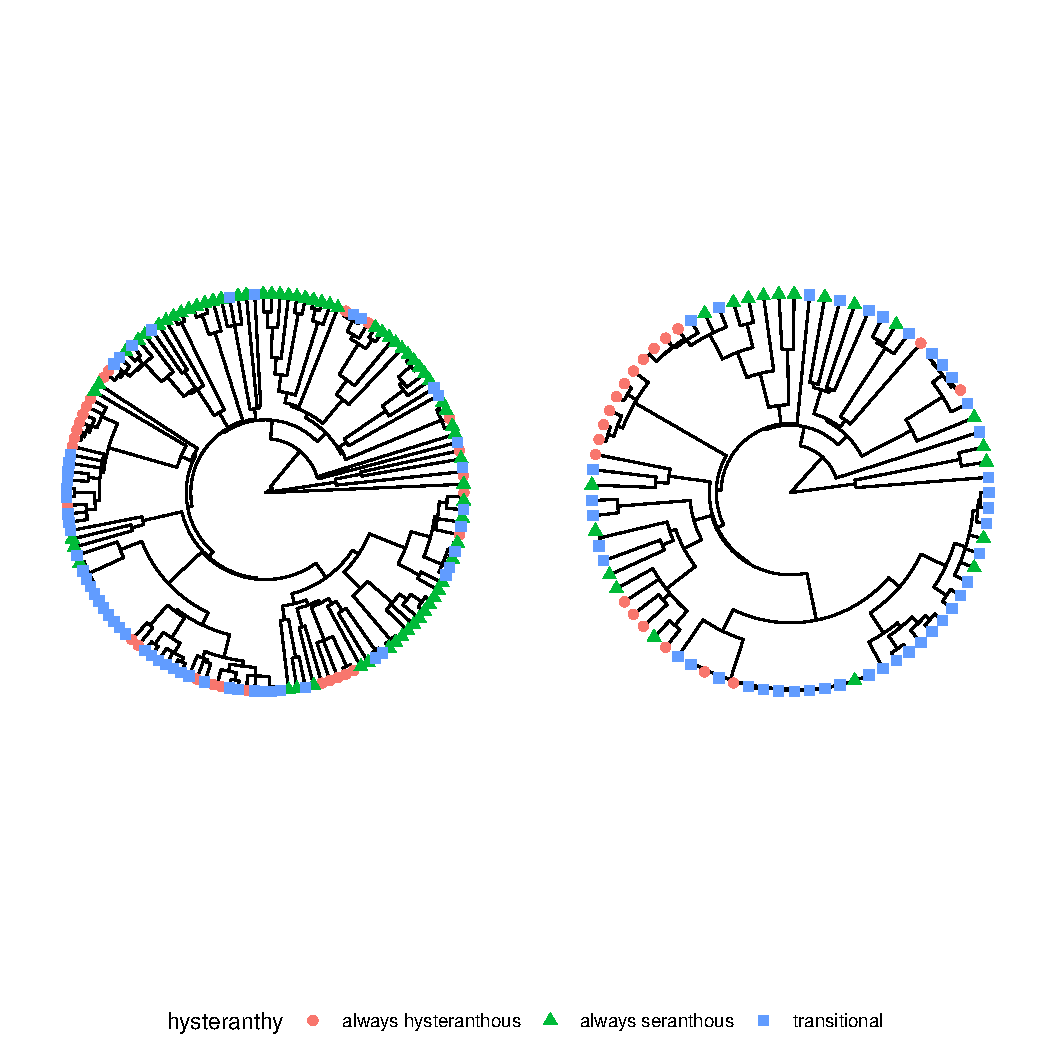
\includegraphics[width=7.5in]{figure/Code_chunk_Minimal_example3-1} 

   
  \caption{\textbf{Phylogenetic structure of FLS in MTSV and USFS varies significantly depending on how FLSs are defined.} Many species get re-assigned to either hysteranthy or seranthy depending on whether FLS is defined functionally (partial overlap between flowering and leafing allowed) or physiologically (no overlap between flowering and leafing allowed) (blue squares). This modeling choice dramatically alters FLS patterning across the tree, resulting in an unstable phylogentic signal for this trait.}
    \label{fig:phylogeny}
    \end{figure}
  
  
\clearpage

\bibliography{..//refs/hyst_outline.bib}[H]
\end{document}
